\documentclass{article}

\usepackage{amsmath, amsthm, amssymb, amsfonts}
\usepackage{thmtools}
\usepackage{graphicx}
\usepackage{setspace}
\usepackage{geometry}
\usepackage{float}
\usepackage{hyperref}
\usepackage[utf8]{inputenc}
\usepackage[english]{babel}
\usepackage{framed}
\usepackage[dvipsnames]{xcolor}
\usepackage[most]{tcolorbox}
\usepackage{minted}
\usepackage{enumitem}
\usepackage{booktabs}
\usepackage{multirow}
\usepackage{amsmath}
\usepackage{caption}     
\usepackage{subcaption}
\usepackage[normalem]{ulem}

\usepackage{indentfirst}

\usepackage[export]{adjustbox} % Align images

\colorlet{LightGray}{White!90!Periwinkle}
\colorlet{LightOrange}{Orange!15}
\colorlet{LightGreen}{Green!15}

\newcommand{\HRule}[1]{\rule{\linewidth}{#1}}

\newtcbtheorem[auto counter,number within=section]{code}{Código}{
  colback=LightOrange!20,
  colframe=LightOrange,
  colbacktitle=LightOrange,
  fonttitle=\bfseries\color{black},
  boxed title style={size=small,colframe=LightOrange},
}{code}

\setstretch{1.2}
\geometry{
  textheight=22.5cm,
  textwidth=13.75cm,
  top=2.5cm,
  headheight=12pt,
  headsep=25pt,
  footskip=30pt
}

\DeclareMathOperator*{\argmax}{argmax}
% ------------------------------------------------------------------------------

\begin{document}

% ------------------------------------------------------------------------------
% Cover Page and ToC
% ------------------------------------------------------------------------------
\begin{center}
  \begin{figure}
    
\includegraphics[scale = 0.3, left]{img/IST_A.eps} % IST logo
    \end{figure}
  \LARGE{ \normalsize \textsc{} \\
  [2.0cm] 
  \LARGE{ \LARGE \textsc{Machine Learning}} \\
  [1cm]
  \LARGE{ \LARGE \textsc{LEIC IST-UL}} \\
  [1cm]
  \HRule{1.5pt} \\
  [0.4cm]
  \LARGE \textbf{\uppercase{Relatório - Homework 1}}
  \HRule{1.5pt}
  \\ [2.5cm]
  }
\end{center}

\begin{flushleft}
  \textbf{\LARGE Grupo 10:}
\end{flushleft}

\begin{center}
  \begin{minipage}{0.7\textwidth}
      \begin{flushleft}
        \large Gabriel Ferreira \\
        \large  Irell Zane
      \end{flushleft}
  \end{minipage}%
  \begin{minipage}{0.3\textwidth}
      \begin{flushright}
        \large 107030\\
        \large 107161
      \end{flushright}
  \end{minipage}
\end{center}

\begin{center}
  \vspace{4cm}
  \date \large \bf  2024/2025 -- 1st Semester, P1
\end{center}

\setcounter{page}{0}
\thispagestyle{empty}
\renewcommand{\thesection}{\Roman{section}}

\newpage

% ------------------------------------------------------------------------------
% Content
% ------------------------------------------------------------------------------



\large{\textbf{Part I}: Pen and paper}\normalsize




\begin{enumerate}[leftmargin=\labelsep]
\item F1-measure of a kNN.


\begin{table}[H]
  \centering
  \begin{tabular}{c|cccc|cccc|}
    \multicolumn{1}{c}{} & \multicolumn{4}{c}{P} & \multicolumn{4}{c}{N}  \\
      & x1 & x2 & x3 & x4 & x5 & x6 & x7 & x8  \\ \hline
  x1  & -  & 2  & 1  & 0  & 1  & 1  & 1  & 2   \\
  x2  & 2  & -  & 1  & 2  & 1  & 1  & 1  & 0   \\
  x3  & 1  & 1  & -  & 1  & 2  & 2  & 0  & 1   \\
  x4  & 0  & 2  & 1  & -  & 1  & 1  & 1  & 2   \\
  x5  & 1  & 1  & 2  & 1  & -  & 0  & 2  & 1   \\
  x6  & 1  & 1  & 2  & 1  & 0  & -  & 2  & 1   \\
  x7  & 1  & 1  & 0  & 1  & 2  & 2  & -  & 1   \\
  x8  & 2  & 0  & 1  & 2  & 1  & 1  & 1  & -   \\ \hline
  \end{tabular}
  \caption{Hamming distance between observations}
\end{table}


Thus with $k = 5$, and a leave-one-out evaluation schema,
we use the closest 5 observations for each, excluding itself,
to calculate the estimate using a weighted mode like so:

\begin{equation*}
  f(x_{new}) \leftarrow \argmax_{c \in \{P, N\} } \sum^i w_i \cdot \delta(c, f(x_i))
\end{equation*}

\begin{equation*}
  w_i = \begin{cases}
    \frac{1}{d(x_new, x_i)} & \text{if\ } x_{new} \neq x_i \\
    1 & else
  \end{cases}
\end{equation*}

In this case, because the relevant observations all
have distances of either 0 or 1, the weight of each
is the same:

\begin{table}[H]
  \centering
  \begin{tabular}{c|cccc|cccc|ccc}
    \multicolumn{1}{c}{} & \multicolumn{4}{c}{P} & \multicolumn{4}{c}{N}  \\
      & x1 & x2 & x3 & x4 & x5 & x6 & x7 & x8 & P & N & $f(x_{new})$ \\ \hline
  x1  & -  & -  & 1  & 0  & 1  & 1  & 1  & -  & 2 & 3 & N \\
  x2  & -  & -  & 1  & -  & 1  & 1  & 1  & 0  & 1 & 4 & N \\
  x3  & 1  & 1  & -  & 1  & -  & -  & 0  & 1  & 3 & 2 & P \\
  x4  & 0  & -  & 1  & -  & 1  & 1  & 1  & -  & 2 & 3 & N \\
  x5  & 1  & 1  & -  & 1  & -  & 0  & -  & 1  & 3 & 2 & P \\
  x6  & 1  & 1  & -  & 1  & 0  & -  & -  & 1  & 3 & 2 & P \\
  x7  & 1  & 1  & 0  & 1  & -  & -  & -  & 1  & 4 & 1 & P \\
  x8  & -  & 0  & 1  & -  & 1  & 1  & 1  & -  & 2 & 3 & N \\ \hline
  \end{tabular}
  \caption{leave-one-out evaluation kNN classifications}
\end{table}

Now the confusion matrix:
\begin{table}[H]
  \centering
  \begin{tabular}{@{}ccc}
    & P & N \\ \midrule 
    P & 1 & 3 \\
    N & 3 & 1 \\
  \end{tabular}
\end{table}

To calculate the F1-Measure we now need Precision and Recall:

\begin{equation*}
  \text{Recall} = \frac{TP}{TP + FN} = \frac{1}{4}
\end{equation*}
\begin{equation*}
  \text{Precision} = \frac{TP}{TP + FP} = \frac{1}{4}
\end{equation*}


\fbox{
  \begin{minipage}{\textwidth}
    \vspace{2pt}
  \textbf{I.1 Solution:}
  
  \begin{equation*}
    \text{F1 Score} = \frac{2}{\frac{1}{P}+\frac{1}{R}} = \frac{2}{4+4} = \frac{\textbf1}{\textbf4}
  \end{equation*}
  \vspace{2pt}
\end{minipage}
}

\item An example of a distance and $k$ that will improve 
the F1-Measure by three fold is the following:


\fbox{
  \begin{minipage}{\textwidth}
    \vspace{2pt}
  \textbf{I.2 Solution:}
  \begin{equation*}
    d(x_1, x_2) = 2 \cdot d_{y_1}(x_1, x_2) + d_{y_2}(x_1, x_2)
  \end{equation*}
  \begin{equation*}
    k = 3
  \end{equation*}
  \vspace{2pt}
\end{minipage}
}
\vspace{2pt}

Where $d_{y_j}(x_1, x_2)$ is the Hamming distance between 
$x_1$ and $x_2$ considering only the variable $y_j$.

To demonstrate the same process as previous but with the
new distance measure and $k$ value:

\begin{table}[H]
  \centering
  \begin{tabular}{c|cccc|cccc|}
    \multicolumn{1}{c}{} & \multicolumn{4}{c}{P} & \multicolumn{4}{c}{N}  \\
      & x1 & x2 & x3 & x4 & x5 & x6 & x7 & x8 \\ \hline
  x1  & -  & 3  & 1  & 0  & 2  & 2  & 1  & 2  \\
  x2  & 3  & -  & 2  & 3  & 1  & 1  & 2  & 0  \\
  x3  & 1  & 2  & -  & 1  & 3  & 3  & 0  & 2  \\
  x4  & 0  & 3  & 1  & -  & 2  & 2  & 1  & 2  \\
  x5  & 2  & 1  & 3  & 2  & -  & 0  & 3  & 1  \\
  x6  & 2  & 1  & 3  & 2  & 0  & -  & 3  & 1  \\
  x7  & 1  & 2  & 0  & 1  & 3  & 3  & -  & 2  \\
  x8  & 3  & 0  & 2  & 3  & 1  & 1  & 2  & -  \\ \hline
  \end{tabular}
  \caption{New distance between observations}
\end{table}

\begin{table}[H]
  \centering
  \begin{tabular}{c|cccc|cccc|ccc}
    \multicolumn{1}{c}{} & \multicolumn{4}{c}{P} & \multicolumn{4}{c}{N}  \\
      & x1 & x2 & x3 & x4 & x5 & x6 & x7 & x8 & P & N & $f(x_{new})$ \\ \hline
  x1  & -  & -  & 1  & 0  & -  & -  & 1  & -  & 2 & 1 & P \\
  x2  & -  & -  & -  & -  & 1  & 1  & -  & 0  & 0 & 3 & N \\
  x3  & 1  & -  & -  & 1  & -  & -  & 0  & -  & 2 & 1 & P \\
  x4  & 0  & -  & 1  & -  & -  & -  & 1  & -  & 2 & 1 & P \\
  x5  & -  & 1  & -  & -  & -  & 0  & -  & 1  & 1 & 2 & N \\
  x6  & -  & 1  & -  & -  & 0  & -  & -  & 1  & 1 & 2 & N \\
  x7  & 1  & -  & 0  & 1  & -  & -  & -  & -  & 3 & 0 & P \\
  x8  & -  & 0  & -  & -  & 1  & 1  & -  & -  & 1 & 2 & N \\ \hline
  \end{tabular}
  \caption{leave-one-out evaluation with new metric}
\end{table}

This metric performs better in this data set 
as can be seen in the confusion matrix:

\begin{table}[H]
  \centering
  \begin{tabular}{@{}ccc}
    & P & N \\ \midrule 
    P & 3 & 1 \\
    N & 1 & 3 \\
  \end{tabular}
\end{table}

\begin{equation*}
  \text{Recall} = \frac{TP}{TP + FN} = \frac{3}{4}
\end{equation*}
\begin{equation*}
  \text{Precision} = \frac{TP}{TP + FP} = \frac{3}{4}
\end{equation*}

\begin{equation*}
  \text{F1 Score} = \frac{2}{\frac{1}{P}+\frac{1}{R}} = \frac{2}{\frac{4}{3}+\frac{4}{3}} = \frac{\textbf3}{\textbf4}
\end{equation*}

\vspace{2pt}
\noindent
The original F1 score was $\frac{1}{4}$, and the new F1 score is $\frac{3}{4}$. 

\begin{equation*}
  \frac{\text{New F1}}{\text{Original F1}} = \frac{\frac{3}{4}}{\frac{1}{4}} = 3
\end{equation*}

Thus, the F1 score has indeed improved by a factor of 3.
\item \begin{enumerate}

  \item \textbf{Dataset}:
  \begin{table}[h]
  \centering
  \begin{tabular}{ccccc}
  \toprule
  $x$ & $y_1$ & $y_2$ & $y_3$ & Class \\
  \midrule
  1 & A & 0 & 1.1 & P \\
  2 & B & 1 & 0.8 & P \\
  3 & A & 1 & 0.5 & P \\
  4 & A & 0 & 0.9 & P \\
  5 & B & 0 & 1.0 & N \\
  6 & B & 0 & 0.9 & N \\
  7 & A & 1 & 1.2 & N \\
  8 & B & 1 & 0.9 & N \\
  9 & B & 0 & 0.8 & P \\
  \bottomrule
  \end{tabular}
  \caption{Observed Values}
  \end{table}

  \item \textbf{Priors}:
  \begin{itemize}
      \item For class Positive (P):
      \[
      p(P) = \frac{5}{9}
      \]
      \item For class Negative (N):
      \[
      p(N) = \frac{4}{9}
      \]
  \end{itemize}

  \item \textbf{Class-conditional Probabilities}:
  \begin{itemize}
      \item Calculate the probabilities of the variable set \(\{y_1, y_2\}\) given each class.
      \item The values are calculated as follows:
      \begin{align*}
        p(y_1 = A, y_2 = 0) &= \frac{2}{9} \\
        p(y_1 = A, y_2 = 1) &= \frac{2}{9} \\
        p(y_1 = B, y_2 = 0) &= \frac{2}{9} \\
        p(y_1 = B, y_2 = 1) &= \frac{3}{9} \\
        p(y_1 = A, y_2 = 0 | P) &= \frac{2}{5} \\
        p(y_1 = A, y_2 = 1 | P) &= \frac{1}{5} \\
        p(y_1 = B, y_2 = 0 | P) &= \frac{1}{5} \\
        p(y_1 = B, y_2 = 1 | P) &= \frac{1}{5} \\
        p(y_1 = A, y_2 = 0 | N) &= 0 \\
        p(y_1 = A, y_2 = 1 | N) &= \frac{1}{4} \\
        p(y_1 = B, y_2 = 0 | N) &= \frac{2}{4} \\
        p(y_1 = B, y_2 = 1 | N) &= \frac{1}{4}
      \end{align*}
  \end{itemize}

  \item \textbf{Mean and Standard Deviation of \(y_3\)}:
  \begin{itemize}
      \item For all observations:  
      \begin{align*}
        \mu_{y_3} &= \frac{1.1 + 0.8 + 0.5 + 0.9 + 0.8 + 1.0 + 0.9 + 1.2 + 0.9}{9} \\ 
              &= 0.9
      \end{align*}
      
      \begin{align*}
        \sigma_{y_3} &= \sqrt{\frac{(1.1 - 0.9)^2 + (0.8 - 0.9)^2 + (0.5 - 0.9)^2 + (0.9 - 0.9)^2...}{8}} \\
                  &\approx 0.2
      \end{align*}
      
      \item For Positive (P):
      \begin{align*}
        \mu_{y_3,P} &= \frac{1.1 + 0.8 + 0.5 + 0.9 + 0.8}{5} = 0.82 \\
        \sigma_{y_3,P} &= \sqrt{\frac{(1.1 - 0.82)^2 + (0.8 - 0.82)^2 + (0.5 - 0.82)^2 + ...}{4}} \\
                  &\approx 0.217
      \end{align*}
      
      \item For Negative (N):
      \begin{align*}
        \mu_{y_3,N} &= \frac{1.0 + 0.9 + 1.2 + 0.9}{4} = 1.0 \\
        \sigma_{y_3,N} &= \sqrt{\frac{(1.0 - 1.0)^2 + (0.9 - 1.0)^2 + (1.2 - 1.0)^2 + (0.9 - 1.0)^2}{3}} \\
                  &\approx 0.1414
      \end{align*}

  \end{itemize}

  \item \textbf{Prediction of Class}:
  \begin{itemize}
      \item To predict the class of a new observation \((y_1, y_2, y_3)\), we calculate the probability for both classes (Positive and Negative) and choose the class with the higher probability:
      \[
      \text{Predicted Class} = \argmax_h p(h | y_1, y_2, y_3)
      \]
  \end{itemize}
  
  \begin{align*}
  \text{where } p(h | y_1, y_2, y_3) &= \frac{p(y_1, y_2, y_3 | h) \cdot p(h)}{p(y_1, y_2, y_3)} \\[10pt]
  &= \frac{p(y_1, y_2 | h) \cdot p(y_3 | h) \cdot p(h)}{p(y_1, y_2) \cdot p(y_3)} \\[10pt]
  \text{where } p(y_3 | h) &= \frac{1}{\sigma_h \sqrt{2\pi}} \exp\left(-\frac{(y_3 - \mu_h)^2}{2\sigma_h^2}\right) \\[10pt]
  \text{and } p(y_3) &= \frac{1}{0.2 \sqrt{2\pi}} \exp\left(-\frac{(y_3 - 0.9)^2}{2 \cdot 0.2^2}\right)
  \end{align*}

\end{enumerate}

\item Under a MAP assumption we do not need to calculate the
denominator, thus:
\begin{equation*}
  \text{Predicted Class} = \argmax_h \{ p(y_1, y_2 | h) \cdot p(y_3 | h) \cdot p(h) \}
\end{equation*}
\newpage
\begin{enumerate} 
  \item For observation (A, 1, 0.8):


  For class \( P \):
  \begin{align*}
  p(y_3=0.8 | P) &= \frac{1}{0.217 \sqrt{2\pi}} \exp\left(-\frac{(0.8 - 0.82)^2}{2 \cdot 0.217^2}\right) \\[10pt]
  &= 1.83\\
  p(y_3=0.8) &= \frac{1}{0.2 \sqrt{2\pi}} \exp\left(-\frac{(0.8 - 0.9)^2}{2 \cdot 0.2^2}\right) \\[10pt]
  &= 1.76\\
  p(P) \cdot p(y_1 = A, y_2 = 1, y_3=0.8 | P) &= \frac{5}{9} \cdot \frac{1}{5} \cdot 1.83 \\[10pt]
  &\approx 0.203
  \end{align*}

  
  For class N:
  \begin{align*}
  p(y_3=0.8 | N) &= \frac{1}{0.1414 \sqrt{2\pi}} \exp\left(-\frac{(0.8 - 1.0)^2}{2 \cdot 0.1414^2}\right) \\[10pt]
  &= 1.038\\
  p(N) \cdot p(y_1 = A, y_2 = 1, y_3=0.8 | N)   &= \frac{4}{9} \cdot \frac{1}{4} \cdot 1.038 \\[10pt]
  &\approx 0.115
  \end{align*}
  
  \textbf{
  Since $0.203 > 0.115$, the predicted class is P.
  }

  \item For observation (B, 1, 1):
  
  For class \( P \):
  \begin{align*}
  p(y_3=1 | P) &= \frac{1}{0.217 \sqrt{2\pi}} \exp\left(-\frac{(1 - 0.82)^2}{2 \cdot 0.217^2}\right) \\[10pt]
  &=1.304 \\
  p(y_3=1) &= \frac{1}{0.2 \sqrt{2\pi}} \exp\left(-\frac{(1 - 0.9)^2}{2 \cdot 0.2^2}\right) \\[10pt]
  &= 1.76\\
  p(P) \cdot p(y_1 = B, y_2 = 1, y_3=1 | P) &= \frac{5}{9} \cdot \frac{1}{5} \cdot 1.304 \\[10pt]
  &\approx 0.145
  \end{align*}

  
  For class N:
  \begin{align*}
  p(y_3=1 | N) &= \frac{1}{0.1414 \sqrt{2\pi}} \exp\left(-\frac{(1 - 1.0)^2}{2 \cdot 0.1414^2}\right) \\[10pt]
  &= 2.82\\
  p(N) \cdot p(y_1 = B, y_2 = 1, y_3=1 | N) &= \frac{4}{9} \cdot \frac{1}{4} \cdot 2.82 \\[10pt]
  &\approx 0.313
  \end{align*}
  
  \textbf{
  Since $0.145 < 0.313$, the predicted class is N.
  }

  \item For observation (B, 0, 0.9):
  
  For class \( P \):
  \begin{align*}
  p(y_3=0.9 | P) &= \frac{1}{0.217 \sqrt{2\pi}} \exp\left(-\frac{(0.9 - 0.82)^2}{2 \cdot 0.217^2}\right) \\[10pt]
  &= 1.72\\
  p(y_3=0.9) &= \frac{1}{0.2 \sqrt{2\pi}} \exp\left(-\frac{(0.9 - 0.9)^2}{2 \cdot 0.2^2}\right) \\[10pt]
  &= 1.99\\
  p(P) \cdot p(y_1 = B, y_2 = 0, y_3=0.9 | P) &= \frac{5}{9} \cdot \frac{1}{5} \cdot 1.72 \\[10pt]
  &\approx 0.191
  \end{align*}

  
  For class N:
  \begin{align*}
  p(y_3=0.9 | N) &= \frac{1}{0.1414 \sqrt{2\pi}} \exp\left(-\frac{(0.9 - 1.0)^2}{2 \cdot 0.1414^2}\right) \\[10pt]
  &= 2.20\\
  p(N) \cdot p(y_1 = B, y_2 = 0, y_3=0.9 | N) &= \frac{4}{9} \cdot \frac{2}{4} \cdot 2.20 \\[10pt]
  &\approx 0.489
  \end{align*}
  \textbf{
  Since $0.191 < 0.489$, the predicted class is N.
  }
\end{enumerate}


\centering
\fbox{
  \begin{minipage}{0.7\textwidth}
    \vspace{2pt}
  \textbf{I.4 Solution:}
  \begin{table}[H]
    \centering
    \begin{tabular}{cccc}
      & (A, 1, 0.8) & (B, 1, 1) & (B, 0, 0.9) \\ \midrule
      Class & P & N & N \\
    \end{tabular}
  \end{table}
  \vspace{2pt}
\end{minipage}
}

\newpage

\raggedright
\item Class-conditional frequency of each word in the training vocabulary.

\begin{table}[H]
  \centering
  \begin{tabular}{ccccccccccc}
    c & "Amazing" & "run" & "I" & "like" & "it" & "Too" & "tired" & "bad" & $N_c$ & $V$ \\ \midrule
    P & 1 & 1 & 1 & 1 & 1 & 0 & 0 & 0 & 5 & \multirow{2}{*}{8} \\
    N & 0 & 1 & 0 & 0 & 0 & 1 & 1 & 1 & 4 \\
  \end{tabular}
\end{table}

Under a ML assumption, for the word $w$:

\begin{align*}
  \text{Predicted Class} &= \argmax_c \{ p(c|w) \} \\
  &= \argmax_c \{ \frac{p(w|c) \cdot \hbox{\sout{$p(c)$}}}{\hbox{\sout{$p(w)$}}} \} \\
  &= \argmax_c \{ \prod^ip(t_i|c) \}
\end{align*}


\begin{table}[H]
  \centering
  \begin{tabular}{ccccc|c}
     & "I" & "like" & "to" & "run" & $\prod^ip(t_i|c)$ \\ \toprule
    $freq(t_i | P)$ & 1 & 1 & 0 & 1 & \multirow{2}{*}{$\frac{2^3\cdot 1}{13^4}=0.000280$} \\
    $p(t_i|P)$      & $\frac{1+1}{5+8}$ & $\frac{1+1}{5+8}$ & $\frac{0+1}{5+8}$ & $\frac{1+1}{5+8}$ \\ \midrule
    $freq(t_i | N)$ & 0 & 0 & 0 & 1 & \multirow{2}{*}{$\frac{2\cdot 1^3}{12^4}=0.000096$} \\
    $p(t_i|P)$      & $\frac{0+1}{4+8}$ & $\frac{0+1}{4+8}$ & $\frac{0+1}{4+8}$ & $\frac{1+1}{4+8}$ \\
  \end{tabular}
\end{table}

\textbf{
  Since $0.000280 > 0.000096$, the predicted class is P.
}

\centering
\fbox{
  \begin{minipage}{0.7\textwidth}
    \vspace{2pt}
  \textbf{I.5 Solution:} \\
  \textbf{
    Since $0.000280 > 0.000096$, the predicted class is P.
  }
  \vspace{2pt}
\end{minipage}
}
\end{enumerate}

\large{\textbf{Part II}: Programming}\normalsize

\begin{enumerate}[leftmargin=\labelsep]
\item \begin{enumerate}
    \item Boxplot comparison of the KNN and the Naive Bayes with Gaussian Assumption:
    
    \begin{figure}[H]  % Forces the figure to stay here
        \centering
        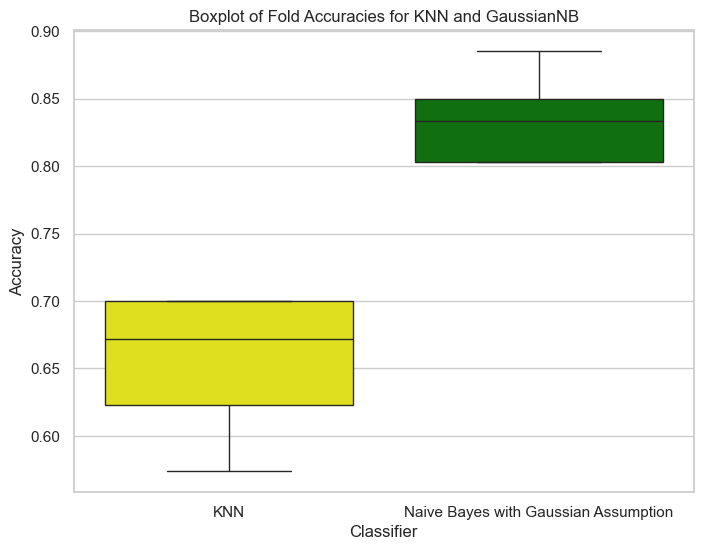
\includegraphics[width=0.8\linewidth]{img/boxplots.png}
        \caption{Boxplots}
        \label{fig:enter-label}
    \end{figure}
    
       The KNN had an overall lower accuracy and was less stable regarding the performance results compared to the Naive Bayes model. This is likely because of the dataset was not scaled. Based on the fact that a knn makes prediction based on the "closest points" to an instance, if the features are on different scales, one feature with a large range will dominate the distance calculation, which can distort the actual "closeness" between points and therefore cause a unstability in the performance of the KNN. 
    
\item 
Original KNN score: 0.65 ± 0.05 \\
KNN score on scaled dataset: 0.82 ± 0.02 \\
Original Naive Bayes score: 0.84 ± 0.03 \\
Naive Bayes score on scaled dataset: 0.84 ± 0.03 \\

The KNN model had significant improvement in accuracy and had more stable results after min-max scaling the dataset. As mentioned in the previous answer the K-nearest neighbour models are sensitive to the scale of the dataset, and scaling can significantly improve the performance of the model. Scaling ensures that all features contribute equally to the distance calculation in the KNN. 

The Naive bayes model with a gaussian assumption had very little to no difference in the results between the scaled and non-scaled data. In the Gaussian model, each feature is modeled separately with its own mean ($\mu$) and variance ($\sigma$) according to the normal distribution. The Naive Bayes model with a Gaussian assumption is insensitive to scaling because this mean and variance are put into consideration when calculating predictions. This explains the indifference in the results.

\item
p1$>$p2? pval= 0.7462688051215336

Through the statistical hypothesis test we received a very high p-value (pval= 0.7462688) and therefore reject the hypothesis asserting that is not true.

\item
Train and test accuracies:

    \begin{figure}[H]
        \centering
        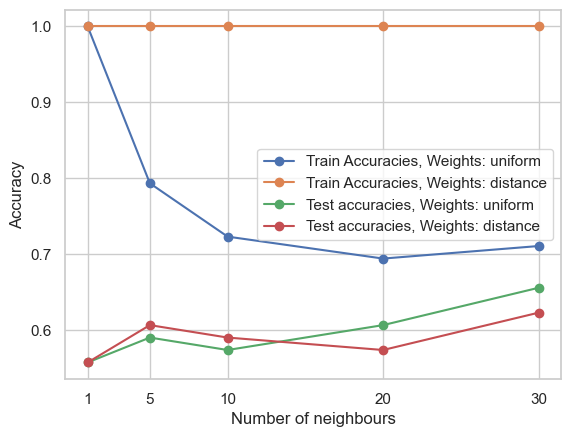
\includegraphics[width=0.8\linewidth]{img/knn_accs.png}
        \caption{KNN accuracies}
        \label{fig:enter-label}
    \end{figure}

\item 
Increasing the number of neighbours, in the knns of both weights (Uniform and Distance), improves the generalization capacity of the model. The model tends to overfit the smaller the number of neighbours parameter is. This is because when you increase n\_neighbors, the model considers more neighboring data points to make a prediction. This therefore prevents overfitting because the decision is based on a larger sample of the training data, rather than on a few close neighbors.

\end{enumerate}

\item
The Naive Bayes model assumes that the features of the data have a distribution similar to that of a normal distribution.
However, some features do not conform to normal distributions well


\begin{figure}[H]
    \centering
    \begin{subfigure}{0.3\linewidth}
        \centering
        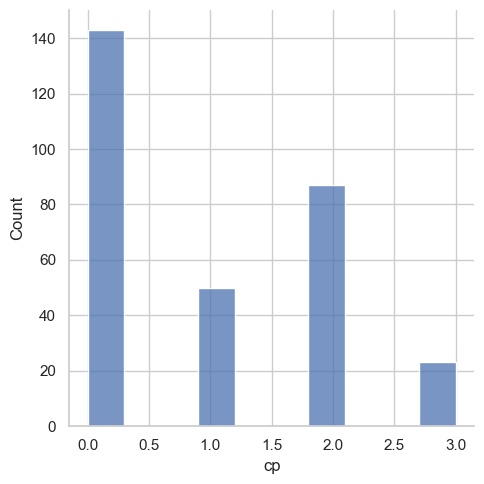
\includegraphics[width=\linewidth]{img/cp_distrib.png}
        \caption{cp feature distribution}
        \label{fig:cp}
    \end{subfigure}
    \hfill % Add horizontal space between subfigures
    \begin{subfigure}{0.3\linewidth}
        \centering
        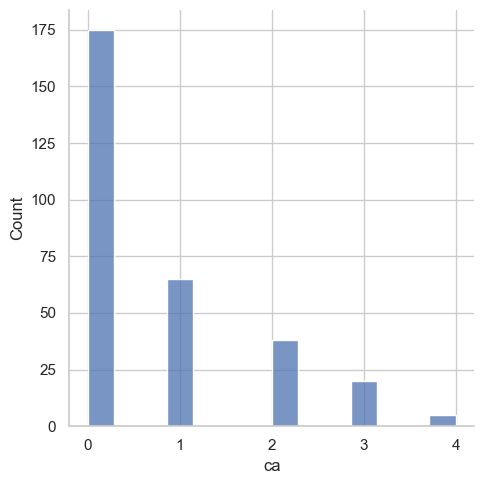
\includegraphics[width=\linewidth]{img/ca_distrib.png}
        \caption{ca feature distribution}
        \label{fig:ca}
    \end{subfigure}
    \hfill % Add horizontal space between subfigures
    \begin{subfigure}{0.3\linewidth}
        \centering
        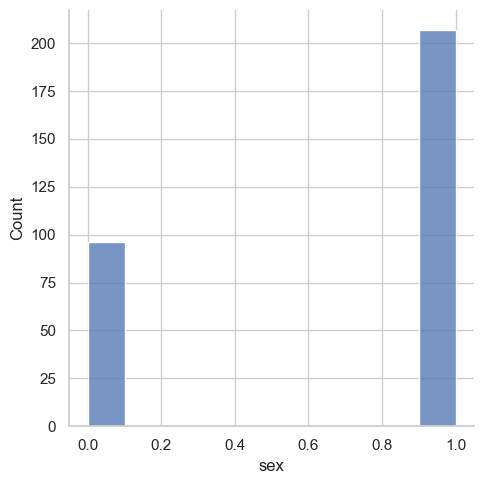
\includegraphics[width=\linewidth]{img/sex_distrib.png}
        \caption{sex feature distribution}
        \label{fig:sex}
    \end{subfigure}
    \caption{Feature distributions}
    \label{fig:distributions}
\end{figure}


The model also assumes that the features are independent to one another. However, some features appear to not be independent to one another.
For example those with heart disease who have sex == 1, seem to tend to have a younger age than those with sex == 0.
\begin{figure}[H]
    \centering
    \begin{subfigure}{0.4\linewidth}
        \centering
        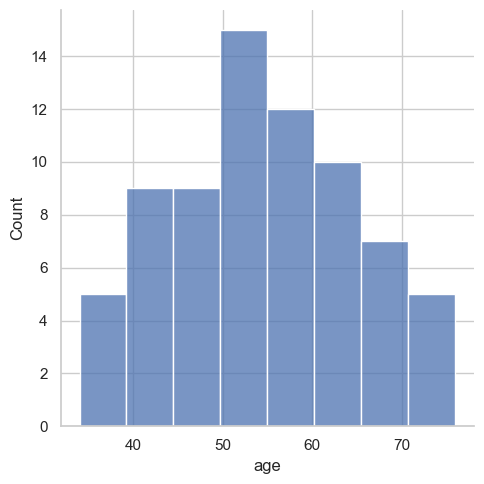
\includegraphics[width=\linewidth]{img/age_sex0.png}
        \caption{age distribution with sex==0}
        \label{fig:cp}
    \end{subfigure}
    \hfill % Add horizontal space between subfigures
    \begin{subfigure}{0.4\linewidth}
        \centering
        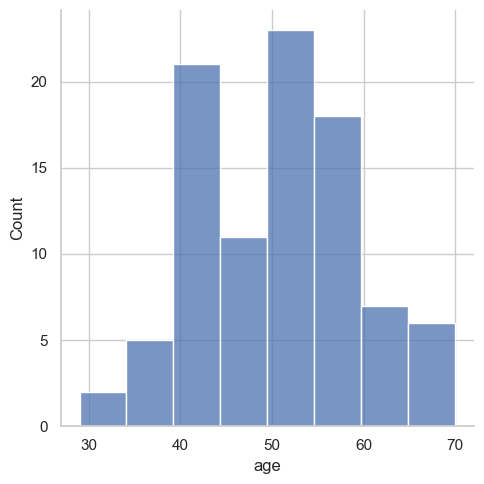
\includegraphics[width=\linewidth]{img/age_sex1.png}
        \caption{age distribution with sex==1}
        \label{fig:ca}
    \end{subfigure}
    \caption{Feature distributions}
    \label{fig:distributions}
\end{figure}

After making a statistical test of such hypothesis and obtaining a pvalue of 0.007 we can say that evidence supports it being true even for common significance levels of $\alpha$ = 0.01.


\end{enumerate}

\vskip 1cm

\newpage

% ----------------------------------------------------------------------
% Cover
% ----------------------------------------------------------------------

\end{document}

